\documentclass[12pt,a4paper,titlepage,openany, oneside]{report}
\usepackage[utf8]{inputenc}
\usepackage[T1]{fontenc}
\usepackage[french]{babel}
\usepackage[top=1.5cm, bottom=4cm]{geometry}
\usepackage{fancyhdr, graphicx, array, hyperref}
\usepackage{glossaries}
%\usepackage[onehalfspacing]{setspace}
%\usepackage{pdfpages}

\pagestyle{fancy}

\title{\textsc{\textbf{Plan projet\\Interpréteur du langage LIR}}}
\date{}
\author{Nicolas \textsc{Caminade} \and Sylvan \textsc{Courtiol} \and
    Pierre \textsc{Debas} \and Heïa \textsc{Dexter} \and Lucàs
    \textsc{Vabre} }
\begin{document}
    \lhead{\leftmark}
    \rhead{
        
\includegraphics[width=2cm]{img/logoiut}
    }

    \cfoot{\thepage}
    \headheight = 2cm
    \headsep = 0.5cm

    \begin{titlepage}
        \fontfamily{pag}\selectfont

        \begin{center}\normalsize
            \MakeUppercase{IUT de Rodez \hfill Département informatique
                \hfill INFO1 2020-2021}
        \end{center}
        \vspace*{0.1cm}
        \hrule
        \vspace*{0.2cm}
        \begin{flushright}
            
\includegraphics[width=4cm]{img/logoiut}
        \end{flushright}
        \vspace*{2cm}
        \begin{flushright}\Huge
            \textsc{\textbf{Plan projet\\Interpréteur du langage LIR}}
        \end{flushright}
        \hrule
        \begin{flushleft}
            \MakeUppercase{Projet proposé par Frédérique Barrios}
        \end{flushleft}
        \vspace*{2cm}
        \begin{center}\Large
            Nicolas \textsc{Caminade}, Sylvan \textsc{Courtiol},\\
            Pierre \textsc{Debas}, Heïa \textsc{Dexter}, \\
            Lucàs \textsc{Vabre}
        \end{center}
        \vfill
        \begin{center}\normalsize
            \MakeUppercase{Projet tuteuré --- Semestre 2}
        \end{center}
    \end{titlepage}

    \renewcommand\rmdefault{pag}
    \fontfamily{pag}\selectfont
    \renewcommand{\sfdefault}{pag}

    % Sommaire
    \renewcommand{\contentsname}{Sommaire}
    \tableofcontents

    \part{Plan projet}

    \chapter*{Introduction}
    \addcontentsline{toc}{chapter}{Introduction}
    \Large
    Dans le cadre des projets tuteuré du semestre 2 de première année de
    DUT informatique de l’année 2020-2021, le sujet de l’Interpréteur LIR
    a été proposé par F. Barrios, un des enseignants de l’IUT de Rodez.
    \\Ce document a pour but de rassembler les informations fondamentales
    relatives à la gestion du projet. Ce plan projet est un document de
    référence du projet qui sera complété tout au long de son avancement.

    \normalsize
    \chapter{Présentation du projet}
    \section{Définition générale du besoin : l'Interpréteur LIR}
    L’Interpréteur LIR est un interpréteur d’un langage de programmation
    simple, il sera nommé LIR pour Langage IUT de Rodez.
    Un interpréteur est un automate enchaînant les tâches suivantes :
    analyse lexico-syntaxique d’une ligne de commande puis interprétation.
    \\Une ligne entrée par un utilisateur sera donc : soit une commande à
    exécuter immédiatement, soit une ligne de programme à mémoriser pour
    une exécution ultérieure. Une ligne de programme se distinguera d'une
    ligne de commande par le fait qu'elle sera toujours précédée d'un
    "numéro d'ordre" appelé aussi "étiquette".

    \section{Cahier des charges}
    Le document en annexe fourni par la maîtrise d’ouvrage (MOA) définit
    l’interpréteur attendu avec les éléments du Langage IUT de Rodez, la
    syntaxe des instructions de programmation et des commandes générales
    attendues dans le logiciel final. Le document précise également le
    comportement attendu de l’interpréteur lors de son utilisation suivi
    d’un exemple d’une session sous cet interpréteur LIR.

    \section{Définitions et acronymes}
        \paragraph{Analyse syntaxique :}
        La vérification de la conformité aux contraintes syntaxiques
        définies par une grammaire.

        \paragraph{Analyse lexicale :}
        L’identification des éléments du vocabulaire d’un langage dans
        une description textuelle (scanning) et la recherche des unités
        lexicales (lexèmes).

        \paragraph{Grammaire :}
        Contraintes syntaxiques définissant les constructions correctes
        (autorisées) d’un langage.

        \paragraph{Interpréteur :}
        Programme capable d’analyser les instructions d’un langage
        (évolué) et de les exécuter directement.

        \paragraph{Langage :}
        Outil de description et d’expression.

        \paragraph{Langage IUT de Rodez (LIR)}

        \paragraph{Sémantique :}
        Étude du sens des unités linguistiques et de leurs combinaisons.
        \\Aspect de la logique qui traite de l'interprétation et de la
        signification des systèmes formels, par opposition à la syntaxe, entendue
        comme l'étude des relations formelles entre formules de tels systèmes
        (d’après le dictionnaire Larousse).

        \paragraph{Syntaxe :}
        Partie de la grammaire qui décrit les règles par lesquelles les unités
        linguistiques se combinent en phrases. En logique, étude des relations
        formelles entre expressions d'un langage (d’après le dictionnaire
        Larousse).
        \\Aussi, la syntaxe est spécifiée par des grammaires et des notations
        formelles.

        \paragraph{Vocabulaire :}
        Symboles de base utilisés dans un langage.

    \section{Charte de projet}
    \subsection{Objectifs du projet}
    Réaliser un interpréteur capable d'exécuter un script ou une série
    d'instructions dans le langage LIR avec les outils et connaissances
    et mis à disposition par l’IUT de Rodez.

    \subsection{Périmètre du projet}
    Ce projet est doit être mené jusqu'à obtention d’un interpréteur
    capable d’exécuter toutes les commandes précisées dans le cahier des
    charges fourni.

    \subsection{Demandes hors périmètre}
    Il n’y a pas de demandes hors périmètre.

    \subsection{Principaux livrables identifiés}
    \paragraph{Livrables :} plan projet, dossier de projet, CD (de
    préférence un dossier compressé plutôt qu’un CD) contenant les codes
    exécutables les fichiers de données, les codes sources et la version
    numérique du dossier et le manuel utilisateur.

    \paragraph{Définition du cadre}
    \subparagraph{Coût :} À définir par le chef de projet (P. Debas).
    \subparagraph{Délais :} Deux dates butoirs identifiées.
        \begin{itemize}
            \item Remise du projet le vendredi 28 mai 2021.
            \item Soutenance du projet la semaine du 7 juin 2021.
        \end{itemize}

    \subparagraph{Qualité :}
    Projet codé en Java dans les respects des conventions et bonnes
    pratiques.

    \subsection{Les acteurs du projet}

    \begin{center}
        \begin{tabular}{rl}
            L'équipe MOE :        & N. CAMINADE, S. COURTIOL, \\
                                  & P. DEBAS, H. DEXTER,      \\
                                  & L. VABRE                  \\
            La MOA :              & F. Barrios                \\
            Le contrôle qualité : & F. Barrios et J. Accot    \\
        \end{tabular}
    \end{center}

    \subsection{Autres moyens et ressources}
    Pas de moyens ou ressources supplémentaires.

    \subsection{Conditions d’acceptation}
    Pas d’exigence ou de contraintes supplémentaires.

    \subsection{Principaux risques identifiés et politique de gestion des risques}
    Si possible tous les membres du groupe auront les mêmes droits sur
    les fichiers communs. En conséquence chaque membre du groupe ne doit
    pas donner des droits sur ces fichiers à une personne extérieure au
    projet (autre que MOA). Cf. Gestion de la configuration (produit par
    S. Courtiol).
    \\Des sauvegardes du dépôt GitHub (contenant toutes les données du
    projets) seront effectuées régulièrement (fréquence à définir) par le
    gestionnaire de configuration. Toutes données qui ne sont pas dans le
    dépôt sont à la responsabilité de chacun. Cf. Gestion de la
    configuration (produit par S. Courtiol).

    \section{Étude générale du besoin}
    \paragraph{Diagramme de cas d'utilisation général de l'Interpréteur LIR}
    comprenant un acteur (le programmeur) et deux cas d'utilisation
    identifiés comme suit :
    \\

    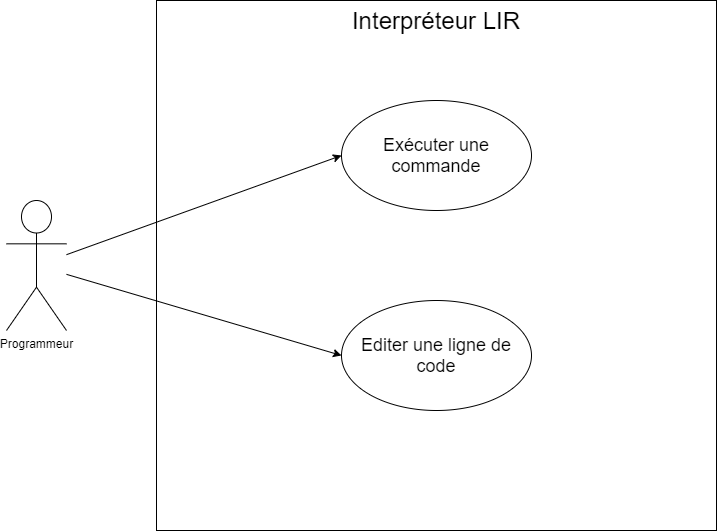
\includegraphics[width=\linewidth]{img/DiagrammeCasUtilisation.png}

    \subsection{Les acteurs}
    \paragraph{Programmeur :} % TODO à détailler
    Personne utilisant l'interpréteur.

    \subsection{Résumés de cas d'utilisation}
    \subsubsection{\Large --- Exécuter une commande}

        \subparagraph{Acteurs}
    Programmeur : il entre une commande à faire exécuter immédiatement par l'interpréteur.

    \subparagraph{Objectifs}
    Exécuter la commande entrée dans l'interpréteur.

    \subparagraph{Pré-Conditions}
    L'interpréteur LIR est lancé et le curseur est derrière l'invite.

    \subparagraph{Post-Conditions}
    La commande est exécutée et un résultat ou un feedback est affiché.

    \subparagraph{Scénario nominal (grandes étapes)}
        \begin{enumerate}
            \item Le programmeur écrit derrière l'invite une ligne de commande.
            \item Le programmeur valide cette commande.
            \item L'interpréteur effectue une analyse lexico-syntaxique.
            \item L'interpréteur interprète la ligne de commande.
        \end{enumerate}

    \subparagraph{Scénarios d'échec}
        \subparagraph{Point 3 du scénario nominal :} la syntaxe de la ligne écrite est incorrecte.
        \begin{itemize}
            \item Un message d'erreur explicite informe le programmeur.
            \item Retour au point 4 du scénario nominal.
        \end{itemize}

        \subparagraph{Point 4 du scénario nominal :} la commande conduit à une erreur d'exécution.
        \begin{itemize}
            \item Un message d'erreur explicite informe le programmeur.
            \item Retour au point 4 du scénario nominal.
        \end{itemize}

%\end{document}

    \subsubsection{\Large --- Éditer une ligne de code}

    
\title{Résumé de cas d'utilisation --- Éditer une ligne de code} % à remplacer


        \subparagraph{Acteurs}
            Programmeur : Il écrit ou modifie une ligne de code dans un
            programme à faire exécuter par l'interpréteur.

        \subparagraph{Objectifs}
            Écrire une une ligne de code dans nouveau programme ou un
            existant afin d'exécuter ou de sauvegarder ce programme.

        \subparagraph{Pré-conditions}
                Le curseur est derrière l'invite suivi d'une étiquette correspondant
                au numéro de la ligne de code à éditer.

        \subparagraph{Post-conditions}
                Le code source édité est prêt à être exécuté, abandonné ou sauvegardé,
                selon l'intention du programmeur.

        \subparagraph{Scénario nominal (grandes étapes)}
            \begin{enumerate}
                \item Le programmeur écrit une instruction ou commande par ligne de code, en la faisant précéder de son étiquette.

                \item Le programmeur consulte le code déjà écrit à tout moment avec la
                      commande \verb|liste|. Selon la syntaxe choisie, l'interpréteur
                      affiche la plage demandée ou la totalité des lignes de code
                      du programme dans l'ordre croissant des étiquettes.

                \item Le programmeur consulte la liste des identificateurs déclarés et
                      leurs valeurs en entrant la commande \verb|defs|.

                \item Au besoin, le programmeur efface une ou plusieurs lignes avec la
                      commande \verb|efface|.

                \item Au besoin, le programmeur efface les lignes de code et identificateurs mémorisés et commence un nouveau code avec la commande \verb|debut|.
            \end{enumerate}

        \subparagraph{Scénarios d'échec}

            \paragraph{Point 2 du scénario nominal :} Aucune ligne de code n'est écrite ou
            la plage de code à afficher n'est pas correcte.
            \begin{itemize}
                \item L'interpréteur en avise le programmeur au moyen d'un message d'erreur.
                \item Retour au point 1.
            \end{itemize}

            \paragraph{Point 3 du scénario nominal :} Aucun identificateur n'a encore été
            déclaré.
            \begin{itemize}
                \item L'interpréteur affiche un message informant le programmeur.
                \item Retour au point 1.
            \end{itemize}

            \paragraph{Point 4 du scénario nominal :} La plage de ligne à effacer est
            incorrecte.
            \begin{itemize}
                \item Un message d'erreur en informe le programmeur
                \item Retour au point 1.
            \end{itemize}


    \subsection{Récits d'utilisation (user stories)}
    Les récits d'utilisation %TODO déf
    \\Des récits d'utilisation ont été rédigés pour chaque commande et instruction.


    \chapter{Organisation du projet}
    \section{Présentation du cycle de vie itératif} % TODO relecture
    Pour développer l’Interpréteur LIR, le modèle de cycle de vie itératif a été
    choisi. Ce modèle de développement de logiciel consiste en une succession de
    cycles de spécification, de conception, de réalisation et de tests, le but
    est d’enrichir et de « remodeler » des prototypes du logiciel successifs. Par
    conséquent, une version du logiciel sera un « dernier prototype ».
    \\La gestion du risque va entraîner la mise en place d’un noyau architectural
    avec des fonctions indispensables du logiciel dès les deux premières
    itérations. Les itérations suivantes apporteront des corrections et de
    nouvelles fonctions au logiciel.
    \\Les versions successives des prototypes permettent de matérialiser
    l’avancement et d’éviter « l’effet tunnel » sur le projet. Ces prototypes
    (versions 0.x) entretiennent la motivation des différents acteurs du projet :
    l’équipe MOE, la MOA.
    \\Le principe fondamental à chaque début d’itération est de ne spécifier en
    détail que les fonctionnalités nécessaires pour cette itération. Ainsi la
    prise en compte d’évolutions du besoin reste possible jusqu'à la dernière
    itération. De même le « refactoring » de la conception (largement facilité
    par les outils) a lieu à chaque étape pour intégrer des évolutions et des
    ajouts. Le but étant bien sûr de fabriquer le logiciel adapté au besoin en
    laissant la possibilité de « mûrir » au cours du temps.
    \\Ce type de cycle implique une taille homogène de l’équipe et une
    polyvalence des équipiers.

    \section{Répartition des rôles}
    Rôles des membres de l’équipe impliqués dans le projet jusqu'au mois de mai
    2021 :
    \begin{center}
        \begin{tabular}{rl}
            Chef de projet MOE            & Pierre Debas      \\
            Secrétaire de projet          & Heïa Dexter       \\
            Gestionnaire de configuration & Sylvan Courtiol   \\
            Développeur                   & Nicolas Caminade  \\
            Développeur                   & Lucàs Vabre       \\
        \end{tabular}
    \end{center}

    \section{Plan communication}
    \subsection{Localisation géographique des intervenants}
    L'équipe MOE, la MOA et les contrôleurs qualités sont basés sur Rodez (12).
    \\La MOA, les contrôleurs qualités, H. Dexter sont basés sur Rodez (12), S.
    Courtiol sur Luc-La-Primaube à côté de Rodez (12), P. Debas est basé à la
    fois sur Rodez et à Albi (81), L. Vabre sur Gages (12) et N. Caminade sur
    Rodez et Moncaut (47).

    \subsection{Moyens de communication utilisés}
    Les communications formelles sont effectuées via les mails de l’IUT
    (généralement par le chef de projet) avec les autres membres du projet en CC.
    \\Serveur Discord spécifique au projet pour communication écrite ou vocale de
    la MOE.
    \\Cf. le document Configuration interpréteur du langage LIR produit par le
    gestionnaire de configuration (S. Courtiol).

    \subsection{Réunions projets MOE}
    Les réunions projet MOE seront hebdomadaires voire bi-hebdomadaires et dans
    le contexte de la crise sanitaire elles se dérouleront en distanciel via
    Discord (vocal, visio-conférence). Seront prévue des réunions courtes de 20
    minutes et des réunions longues de 1h30.
    \\Ces réunions auront pour objectif de faire le point sur l’avancement du
    projet, le respect des objectifs fixé sur la période et de fixer les
    prochains objectifs à remplir d’ici la prochaine réunions. Aussi ces réunions
    seront l’occasion de faire part de difficultés éventuelles rencontrées par
    les membres de l’équipe au cours de la semaine et de communiquer les
    informations sur les prochaines rencontres avec la MOA.
    \\Les comptes-rendus seront rédigés par la secrétaire de projet (H. Dexter)
    et diffusés sur le serveur Discord de l’équipe sous format texte.

    \subsection{Comités de Pilotage}
    Les comités de pilotage rassembleront la MOA et toute l’équipe de MOE. Les
    COPIL seront dirigé par le chef de projet éventuellement assisté par le
    secrétaire.
    \\La fréquence des COPIL est au mieux hebdomadaire et d’une durée d’une
    demi-heure à trois quarts d’heure selon l’avancement du projet.
    Les comptes-rendus des COPIL seront rédigés par l’actuelle secrétaire de
    projet (H. Dexter) et diffusés le lendemain à la MOE du projet.


    \section{Assurance qualité}
    \subsection{Normes et standards de travail à observer (formalisme de modélisation, méthodes de contrôle, méthodes de développement, cycle de vie, conventions de code…)}
    Pour mener à bien ce projet l'équipe MOE travaille
    en utilisant le langage UML comme formalisme de modélisation, la méthode de
    développement dirigé par les tests i.e. la méthode TDD (Test Driven
    Development) en respectant les Java Code Convention pour un modèle de cycle
    de vie itératif.

    %\subsection{Manuel qualité et démarche qualité à observer (suivant la politique qualité de l’organisation), suivi et contrôle qualité (organisation, fréquence, participants).}
    % TODO: À commencer


    \section{Ressources matérielles et logicielles}
        La partie qui suit est un résumé du document de gestion de la configuration joint
        au dossier technique. Merci de vous y référer pour plus de détails.

        La conception en langage UML sera effectuée sous Modelio. La rédaction des
        différents documents du dossier sera faite en utilisant \LaTeX. Nous utiliserons
        Eclipse configuré avec un \emph{workspace} similaire à celui utilisé lors de nos
        cours de programmation. Les dépôts en ligne et le contrôle de l'historique des
        versions seront assurées par Git, plus précisément via GitHub. L'avancement sera
        contrôlé sur un tableau Trello. Enfin, la communication sera assurée via un
        serveur Discord dédié ou Google Meet pour les visio-conférences.

    \chapter{Pilotage du projet}
    \section{Cycle de vie itératif}
    Pour développer l’Interpréteur LIR, le modèle de cycle de vie itératif a été
    choisi. Ce modèle de développement de logiciel, rappelons-le, consiste en une
    succession de cycles de spécification, de conception, de réalisation et de
    tests, le but est d’enrichir et de « remodeler » des prototypes du logiciel
    successifs. Par conséquent, une version du logiciel sera un « dernier
    prototype ».
    \\Si le choix de modèle de cycle de vie s'est porté sur le modèle itératif,
    c'est parce qu'il s'agit d'un modèle "réaliste" et possible à mettre en place
    dans le cadre des projets tuteurés :

    \begin{itemize}
        \item Une limitation de "l'effet tunnel" pour une meilleure dynamique et motivation des équipes (MOA et MOE).
        \item Une meilleure acceptation des changements grâce aux prototypes.
        \item Une meilleure gestion des risques.
        \item Est adapté pour une équipe de cinq personnes polyvalentes.
        \item Le principe d'itérations où seules les fonctionnalités nécessaires sont spécifiées en détail en début d'itération ce qui permet une évolution du besoin.
    \end{itemize}

    \section{Estimation initiale}
        En se focalisant sur un développement de type Organic d'une taille attendue
        de 2000 lignes de code (2KLOC), le projet nécessite de base un effort de 4,97
        mois.homme répartis sur une durée de 4.60 mois. Cette estimation se base sur
        une équipe d'un seul développeur.

        \'{E}tant donné que notre équipe se constitue de 5 personnes, il nous suffit
        d'adapter cette estimation en divisant l'effort par le nombre de membres. Nous
        obtenons ainsi un effort de 0, 99 mois de 20 jours. Notre contexte de travail
        étant toutefois différent de celui d'une entreprise (pas d'horaires fixes,
        travail les jours fériés,...), il nous a paru plus judicieux de convertir
        notre estimation vers un format plus réaliste.

        En considérant une durée de deux heures par journée de travail par personne,
        nous arrivons à un total de 10 heures quotidiennes, soit un total de
        200 heures hebdomadaires. Nous conservons la durée de 20 jours par mois pour
        pallier les indisponibilités de chacun. La durée totale du projet est donc
        estimée à 0,99 mois ou 200 heures de travail total, soit 40 heures.homme.

    \section{Planification prévisionnelle initiale}
        Le développement de l'interpréteur LIR suivant un cycle de vie itératif,
        nous agréé avec la MOA de trois itérations, avec à l'issue de chacune la
        livraison d'un prototype fonctionnel ou, dans le cas de la dernière itération,
        du programme complet.

        Pour la première itération, nous avons convenu de livrer un prototype
        incluant les mécanismes de base du fonctionnement des commandes et instructions.
        Cette première mouture de l'interpréteur Doit être en mesure d'analyser son
        entrée standard, d'affecter des variables de type chaîne à son contexte
        d'exécution et de reconnaître les expressions sur les chaînes de caractères.
        Le contexte pourra être réinitialisé.
        Enfin, ce prototype devra afficher les variables déclarées, afficher le
        résultat d'une expression de type chaîne, et être en mesure
        mettre fin à la session.

        Lors de la seconde itération, notre prototype devra, en plus des fonctionnalités
        sus-mentionnées, incorporer l'affectation de variables de type entier
        et l'arithmétique entière sur les expressions. L'interpréteur, à ce stade du
        développement, devra être en mesure de reconnaître des étiquettes de ligne de
        code et garder en mémoire centrale un programme pour pouvoir ensuite l'afficher ou
        l'exécuter. Il doit également être en mesure de supprimer des lignes de code dans
        le programme global. Il sera également possible à l'utilisateur de saisir puis
        d'affecter la valeur d'une variable via l'entrée standard ou d'effectuer des sauts
        non-conditionnels dans un programme.

        Enfin, le programme final de la troisième itération pourra lire et écrire des
        programmes vers et depuis des fichiers. Il sera possible au programmeur d'effectuer
        des sauts conditionnels. Seront livrés avec ce prototype final ce plan de projet
        complété, ainsi que le manuel d'utilisateur de l'interpréteur LIR. Le prototype
        final devra pouvoir être lancé à partir d'un fichier exécutable.

    \section{Durée et ordonnancement des principales tâches et itérations}
        Afin d'avoir un interpréteur LIR fonctionnel, nous avons identifié un jeu de
        tâches critiques devant être remplies à chaque itération. Ainsi, pour la
        présentation du premier prototype, devront être implémentés et testés les
        littéraux, les identificateurs, les variables, le contexte d'exécution, les
        commandes et instructions, et l'analyseur lexicale.

        Lors de la deuxième itération, devront être traités en priorité la gestion des
        étiquettes et l'implémentation de programmes à stocker en mémoire. Enfin,
        l'analyseur devra prendre en compte cette nouvelle fonctionnalité et référencer
        le programme global de la session.

        Pour finir, la troisième itération consistera à rajouter la possibilité au
        programmeur d'effectuer des sauts conditionnels. Pour ce faire, les conditions
        devront être traitées sous la forme d'une expression booléenne simple. Cela
        implique donc la création d'un littéral de type booléen, non accessible directement
        au programmeur dans cette version de l'interpréteur (le programmeur ne pourra donc
        pas créer de variable de type Booléen). La troisième itération se terminera par
        la revue du code et des jeux de tests, l'édition du manuel utilisateur, ainsi que
        la complétion du dossier technique.

    \section{Identification des premiers jalons}
        Chacun des prototypes de l'interpréteur LIR devant être livré à l'issue de chaque
        itération, nous pouvons donc en déduire les premiers jalons ci-dessous. La date de
        soutenance du projet, quand à elle, nous sera précisée à une date ultérieure à
        la rédaction de ce plan. Nous ne pouvons donc en donner qu'une estimation.

        \begin{itemize}
            \item Premier entretien MOA / MOE et lancement du projet :
                  jeudi 8 avril
            \item Livraison du premier prototype : lundi 10 mai
            \item Livraison du deuxième prototype : mercredi 19 mai
            \item Livraison du prototype final : Vendredi 28 mai
            \item Soutenance du projet : entre le 9 et je 11 juin
        \end{itemize}

    \section{Calendrier prévisionnel}
        \`{A} partir des dates citées plus haut, nous pouvons donc en déduire le
        calendrier prévisionnel suivant. Les comités de pilotage ont été convenus avec
        la maîtrise d'ouvrage afin de conserver un suivi le plus régulier possible sur
        l'avancement du développement.
        \begin{itemize}
            \item Première itération : du 3 au 10 mai
            \item Deuxième itération : du 11 au 19 mai
            \item Comité de pilotage : mardi 18 mai
            \item Troisième itération : du 20 au 28 mai
            \item Comité de pilotage : mercredi 26 mai
            \item Remise du dossier technique : mardi 8 juin
        \end{itemize}

    \section{Organisation des réunions projets et comités de pilotage}
        Comme mentionné, les comités de pilotage se tiennent entre deux livraisons
        afin de faire le point sur l'avancement de l'itération. Compte tenu des restrictions
        sanitaires imposées au cours de la crise due à la Covid-19, nous devrons adapter
        ces réunions aux modalités de présence imposées par l'IUT de Rodez. Selon la
        semaine, certains membres de l'équipe devront y assister en visio-conférence.

        Les réunions de projet, quand à elles, se tiennent à chaque fois qu'un ensemble de
        tâches est complété pour mettre en commun le travail effectué et faire le point sur
        les difficultés techniques rencontrées et la répartition des ressources sur les
        tâches restantes (nous privilégions en effet le travail en binôme et faisons en
        sorte que chaque membre de l'équipe ait l'occasion de travailler au moins une fois
        avec tous les autres).

    \section{Suivi du projet pour la première itération}

    \subsection{Planification et ordonnancement des tâches}
        Au tâches déjà spécifiées dans la section \hyperref{Durée et ordonnancement des principales tâches et itérations}, nous souhaiterions ajouter quelques
        fonctionnalités de base de l'interpréteur LIR. La planification de cette itération
        comprend donc l'implémentation et le test des commandes \verb|defs|, \verb|debut|
        et \verb|fin|, ainsi que des instructions \verb|affiche| et \verb|var|.

        Ce premier prototype fonctionnera uniquement avec des données de type chaîne
        de caractère. Cela implique donc l'ajout d'identificateurs, de constantes
        littérales et d'expressions correspondants.

        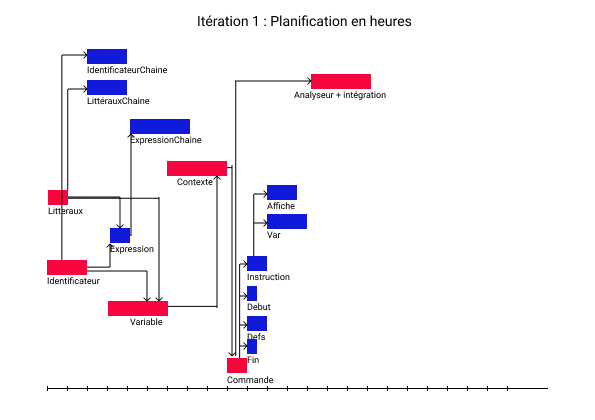
\includegraphics[scale=0.75]{fichiers/planification/iteration1/iteration1Planif.png}

        Le diagramme de planification de l'itération 1 suggère un total de 27 heures de
        travail, soit l'équivalent de 10 jours.homme. En raison du nombre limité de
        ressources de travail, toutes les tâches, notamment les instructions et commandes,
        ne pourront être réalisées en concomitance. Certaines devront donc se voir
        repousser le temps qu'un binôme se libère.



    \subsection{Suivi d’avancement et mesure des écarts par rapport au prévisionnel}

        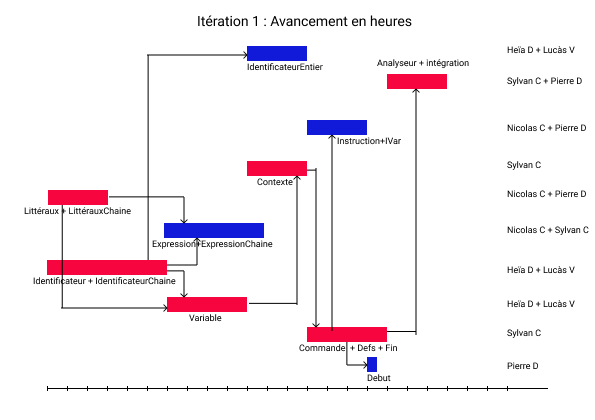
\includegraphics[scale=0.75]{fichiers/planification/iteration1/iteration1Avancement.png}

        \`{A} l'issue de cette première itération, nous constatons un volume de travail
        total de 35 heures, soit 8 heures ou 4 jours.homme de plus que ce qui était
        estimé. Cet écart s'explique d'une part dans une estimation trop optimiste de la
        durée des tests unitaires d'une part et un manque d'habitude à travailler en
        binôme d'autre part. Cette itération portant sur des aspect structurels importants
        de l'interpréteur, il nous sera plus aisé à l'avenir de rajouter les commandes
        et instructions.

%    \subsection{Synthèse par "tableau de bord"}

    \subsection{Résultats des tests et recette de prototype de la période}

%    \subsection{Résultats des revues/suivis/contrôles qualité de la période}

    \subsection{Identification des principaux écarts et problèmes constatés, solutions possibles}
        \`{A} l'issue de cette première période, nous avons pu livrer un prototype
        fonctionnel et ce malgré des difficultés liées à la conception. En revanche,
        l'instruction \verb|affiche|, initialement prévue pour cette itération, n'a
        pas été implémentée, faute de temps et de ressources disponibles, et a donc été
        reportée à l'itération suivante. Cette instruction n'étant pas critique pour
        le fonctionnement de l'application, nous pouvons donc considérer la gravité
        de ce retard comme minime.

    \subsection{Propositions de modification de la planification prévisionnelle pour tenir compte des corrections à apporter}
        Afin de tenir compte de ce léger retard, nous rajouterons l'implémentation de
        l'instruction \verb|affiche| aux tâches à réaliser pour la prochaine itération.
        En plus des programmes, et l'adaptation de l'analyseur à interagir avec, nous en
        profiterons pour implémenter un maximum de fonctionnalités, ce qui nous permettra
        de rattraper le léger retard pris sur la planification originelle.

        Nous laisserons toutefois l'instruction \verb|si..vaen| et les expressions
        conditionnelles qu'elle utilise de côté. En effet, ces dernières nécessiteront
        probablement un \emph{refactoring} de la classe Expression et de ses dérivées.

        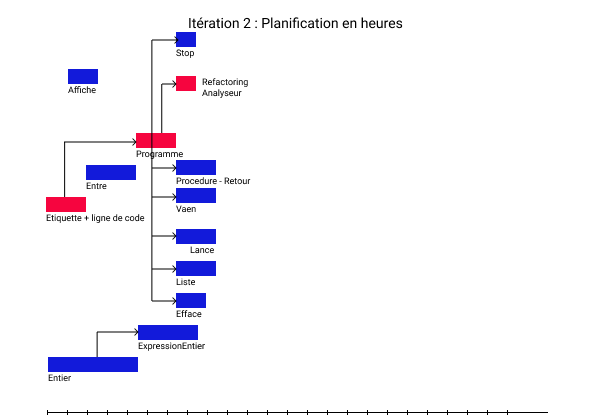
\includegraphics[scale=0.75]{fichiers/planification/iteration2/iteration2Planif.png}

        En suivant la planification ci-dessus, la deuxième itération devrait donc occuper
        un total de 26 heures de travail, soit une durée similaire à la précédente.
        L'objectif du prochain prototype sera de rajouter la majorité des fonctionnalités
        de l'interpréteur LIR, dont notamment l'arithmétique entière et toute la partie
        d'édition et d'exécution de programmes.

    \subsection{Comptes-rendus des réunions projets de la période}
       Voir
       \begin{itemize}
           \item Compte rendu de la réunion MOE du 15 avril
           \item Compte rendu de la réunion MOE du 19 avril
           \item Compte rendu de la réunion MOE du 22 avril
           \item Compte rendu de la réunion MOE du 26 avril
       \end{itemize}

    \subsection{Compte-rendu du comité de pilotage de la période}
        Voir
        \begin{itemize}
            \item Compte rendu de la réunion MOA du 4 mai
            \item Compte rendu de la réunion MOA du 10 mai
        \end{itemize}

    \subsection{Planification prévisionnelle révisée pour les périodes suivantes (en fonction des décisions prises)}
        Exception faite de l'ajout de \verb|affiche|, la planification de la
        deuxième itération ne dévie pas de l'ordonnancement initial. Elle a donc
        été entérinée à l'unanimité.

    \section{Suivi du projet pour la seconde itération}

    \subsection{Suivi d’avancement et mesure des écarts par rapport au prévisionnel revu lors de la période précédente}

    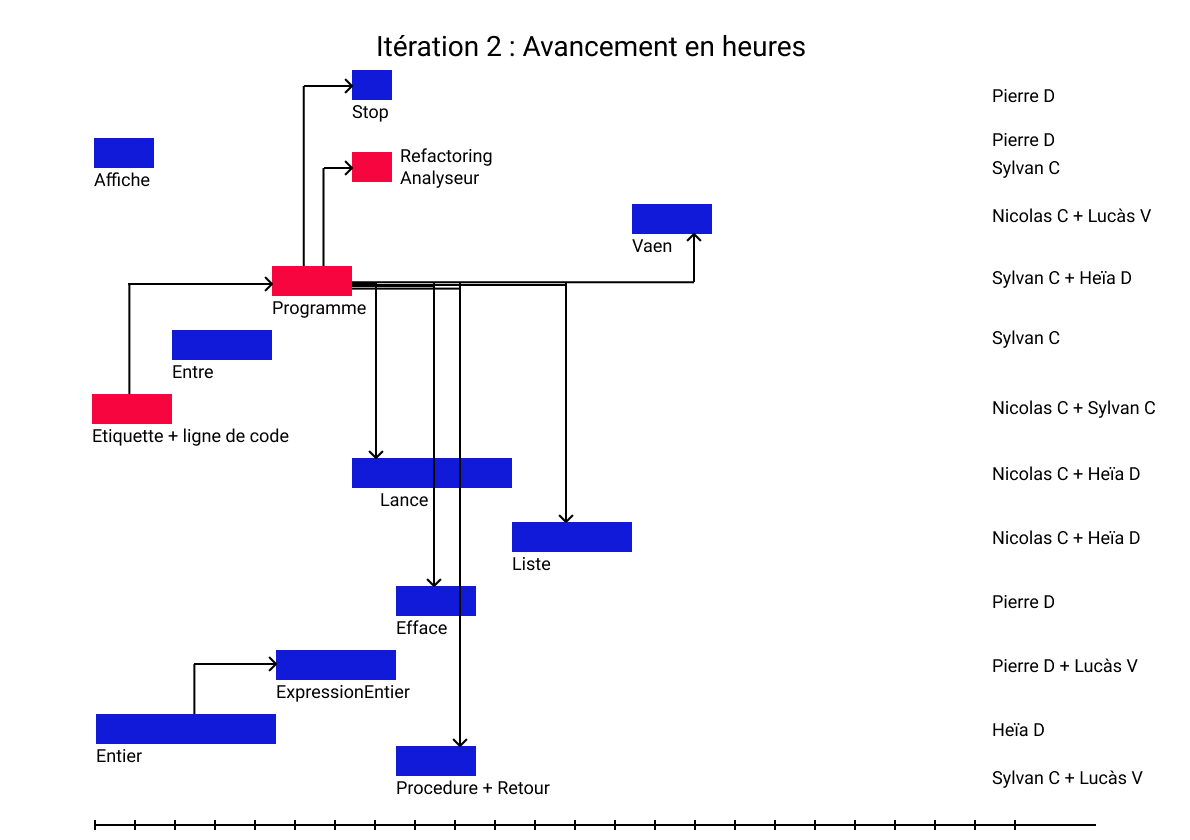
\includegraphics[scale=0.75]{fichiers/planification/iteration2/iteration2Avancement.png}

    Au total, la seconde itération aura englobé un temps de travail total de 30,5 heures,
    soit 4,5 heures ou 2,25 jours.homme de retard par rapport à la planification initiale. Ce
    retard s'explique dans des difficultés à gérer les dépendances avec la classe Programme
    et à écrire des tests concluants. Les instructions \verb|lance| et \verb|liste| sont
    celles nous ayant posé le plus de problèmes.

    Nous pouvons également remarquer, à travers ce graphe, l'étalement dans le temps
    des tâches comparé à la planification précédente. Cela est dû à un inconvénient du
    travail en binôme. En effet, le nombre de membres de notre équipe étant fini, il nous
    a fallu par moments attendre que certains se libèrent d'une tâche pour entamer la
    suivante.

    En entreprise, cet inconvénient est en général mitigé par la quotité horaire
    fixe et convenue dans le contrat de travail. Dans le cadre d'un travail étudiant, nous
    avons aussi dû jouer avec les disponibilités de chacun, en plus des contraintes
    imposées par le travail à deux. En dépit de ces facteurs, nous n'avons aucun écart
    majeur à déplorer dans notre ordonnancement.

    %\subsection{Synthèse par "tableau de bord"}

    \subsection{Résultats des tests et recette de prototype de la période}

    %\subsection{Résultats des revues/suivis/contrôles qualité de la période}

    \subsection{Identification des principaux écarts et problèmes constatés, solutions possibles}
        \`{A} ce stade du projet, aucun gros écart n'est constaté. Nous avons cependant
        été confrontés à des difficultés à mener nos tests correctement, ce qui a fait
        augmenter la durée de certaines tâches (non critiques).

    \subsection{Propositions de modification de la planification prévisionnelle pour tenir compte des corrections à apporter}
        La seconde itération n'ayant pas pris de retard, aucune modification ne sera
        apportée à la planification de la troisième. Le dernier prototype inclura donc
        toutes les fonctionnalités manquantes à ce stade, à savoir la lecture et l'écriture
        de fichiers textes pour la sauvegarde de programmes, ainsi que les expressions
        et sauts conditionnels. Nous profiterons du temps restant pour effectuer une
        revue générale du code et des jeux de tests, rédiger le manuel d'utilisation et
        achever ce plan projet.

    \subsection{Comptes-rendus des réunions projets de la période}
        Voir Compte rendu de la réunion MOE du 11 mai
    \subsection{Compte-rendu du comité de pilotage de la période}
        Voir
        \begin{itemize}
            \item Compte rendu de la réunion MOA du 10 mai
            \item Compte rendu de la réunion MOA du 18 mai
            \item Compte rendu de la réunion MOA du 19 mai
        \end{itemize}


    \subsection{Planification prévisionnelle révisée pour les périodes suivantes (en fonction des décisions prises)}

    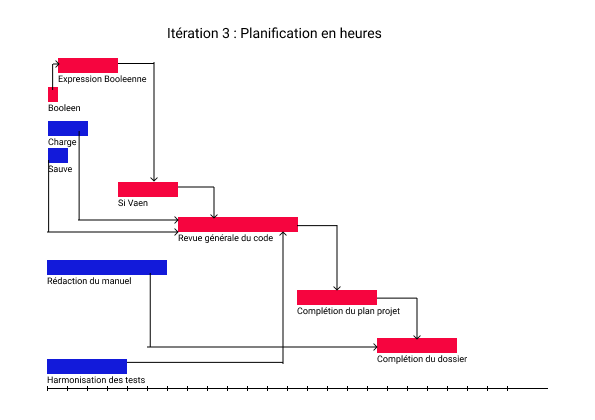
\includegraphics[scale=0.75]{fichiers/planification/iteration3/iteration3Planif.png}

    Au vu des estimations effectuées, la troisième itération devrait couvrir un temps
    de travail de 33,5 heures, soit 16,75 jours.homme. Cette itération comportant de
    nombreuses tâches critiques (le 28 mai marquant le dernier jalon de la phase de
    développement et la livraison du prototype final), nous avons délibérément pris des estimations potentiellement larges
    afin de nous assurer suffisamment de temps pour mener ces tâches à bien.

    \section{Suivi du projet pour la troisième itération}

    \subsection{Suivi d’avancement et mesure des écarts par rapport au prévisionnel revu lors de la période précédente}

    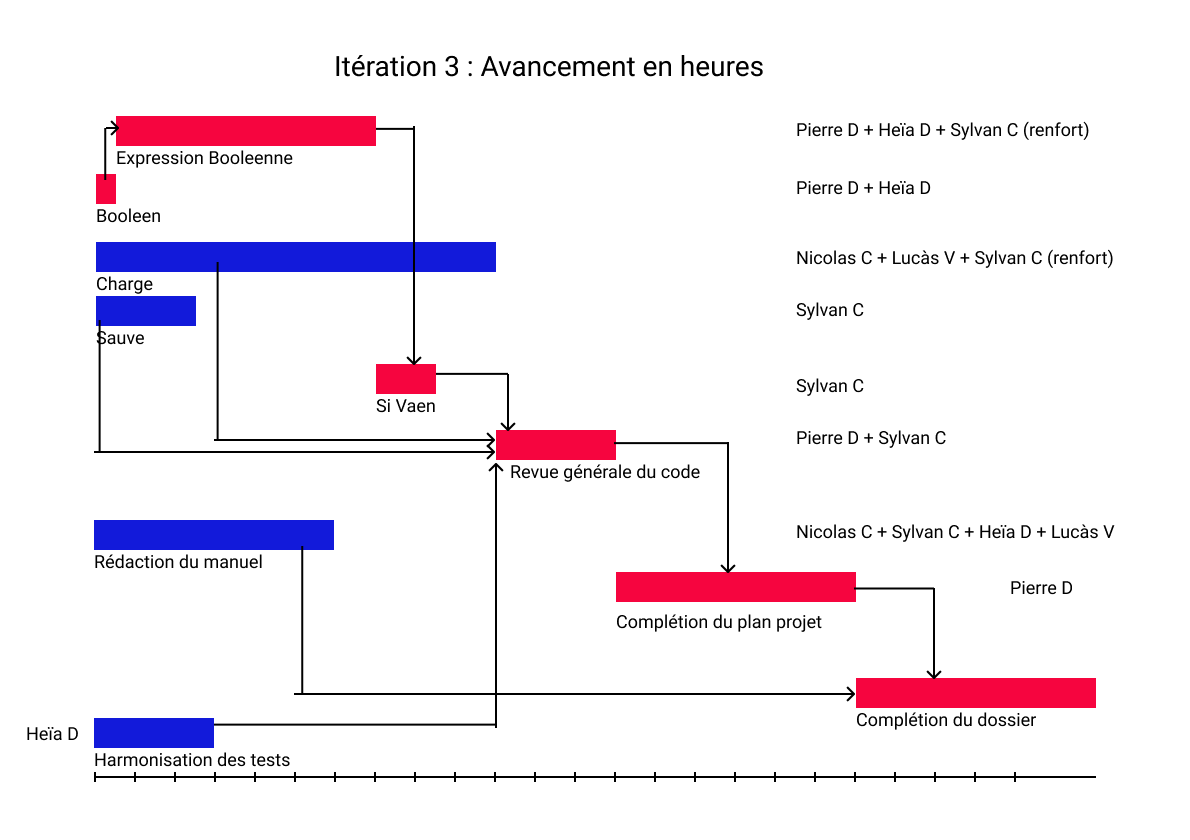
\includegraphics[scale=0.75]{fichiers/planification/iteration3/iteration3Avancement.png}

    Cette troisième itération offre un total d'heures de travail porté à 45 contre les
    33,5 prévues. Cela équivaut donc à un retard de 11,5 heures, soit l'équivalent de
    5,75 jours.homme. Ce retard s'explique par deux problèmes d'envergure auxquels
    nous avons été confrontés. Ces deux problèmes ont eu un impact direct sur le
    cheminement critique de l'ordonnancement et a par conséquent entraîné un retard qu'il a fallu compenser dans la revue de code. Nous reviendrons plus en détail sur ces
    problèmes un peu plus bas.

    %\subsection{Synthèse par "tableau de bord"}

    \subsection{Résultats des tests et recette de prototype de la période}

    %\subsection{Résultats des revues/suivis/contrôles qualité de la période}

    \subsection{Identification des principaux écarts et problèmes constatés, solutions possibles}

    Le premier des deux problèmes mentionnés plus haut concerne l'écriture des
    algorithmes de reconnaissance des expressions booléennes. Ce problème aurait pu
    être évité via l'usage d'expressions rationnelles (\emph{regex}). Malheureusement,
    cette notion est arrivée tard dans notre apprentissage de la théorie des langages et
    nous n'avons pas eu l'opportunité de pouvoir l'implémenter à temps.

    Le deuxième problème, plus grave, a concerné le fonctionnement de la commande charge.
    Il nous est apparu en effet que la plupart du code de cette commande réutilisait celui
    de la classe Analyseur. Il nous est alors apparu une faiblesse dans notre conception,
    étant donné que si ce code est réutilisé à cet endroit, cela signifie qu'une
    factorisation a été mal faite. Une solution serait de repenser l'analyseur comme un
    objet chargé d'analyser une seule ligne de code et de le dissocier de la
    \verb|mainLoop()| de l'interpréteur.

    Malheureusement, cette conclusion ne nous est
    arrivée que tardivement et il a fallu que nous prissions une décision. Nous avons
    donc opté pour la solution la moins coûteuse en durée afin de ne pas accumuler de
    retard et de pouvoir terminer le projet dans les temps. Dans une hypothétique phase
    de maintenance du logiciel, nous pensons qu'implémenter la solution évoquée ci-dessus
    serait une des premières tâches à accomplir dans le but de proposer un logiciel
    fonctionnel et plus facilement maintenable.


    \subsection{Comptes-rendus des réunions projets de la période}

    \subsection{Compte-rendu du comité de pilotage de la période}
        Voir
        \begin{itemize}
            \item Compte rendu de la réunion MOA du 18 mai
            \item Compte rendu de la réunion MOA du 19 mai
        \end{itemize}

    \subsection{Idées d'améliorations}
        L'interpréteur LIR que nous livrons à l'issue de ce projet respecte les
        spécifications du cahier des charges. Au cours de sa conception et de son implémentation, nous nous
        sommes efforcés, avec plus ou moins de succès, à conserver un code le plus
        simple et réutilisable possible, en accord avec l'état de nos connaissances et
        de notre expérience du développement logiciel à cette période de notre formation.

        Afin de rapprocher davantage notre travail de que l'on pourrait attendre d'une
        équipe professionnelle, nous avons réfléchi à un bagage de connaissances et de
        savoirs faire dont nous aurions souhaité disposer dès les premiers instants de la
        conception. Ce dernier nous permettra à l'avenir de surmonter plus facilement
        les difficultés auxquelles nous avons été confrontés.

        D'abord, l'utilisation du \emph{pattern matching} et des expressions
        rationnelles citées plus haut nous aurait grandement simplifié la conception et
        surtout le codage de notre analyseur. Nous ne nous priverons d'ailleurs pas de
        nous en servir lors de projets ultérieurs.

        De plus, l'étude des \emph{design patterns}, des structures de données et de leur
        usage nous simplifiera grandement la tâche de la conception à l'avenir. Avec le
        recul que nous a procuré cette expérience, nous constatons que nous aurions
        pu être bien plus efficaces lors des phases de conception avec ces outils.

        Ensuite, les tests que nous avons réalisés l'ont été avec l'exécuteur universel
        développé au cours des TDs de programmation du deuxième semestre. Si cet outil
        ne nous a à aucun moment fait défaut, nous lui aurions certainement préféré JUnit3.
        Sachant que les tests occupent au moins la moitié de la phase de développement d'un
        logiciel, nous aurions certainement gagné en efficacité avec cet outil.

        Pour finir et pour aller plus loin, à présent que l'interpréteur fonctionne, il
        pourrait être intéressant, comme projet d'été par exemple, de développer un
        IDE dédié à notre interpréteurLIR. Cette application proposerait une interface
        fenêtrée, l'autocomplétion, l'utilisation des commandes à travers des
        menus déroulants ou encore l'affichage du contexte en temps réel.


    \chapter{Bilan}
        \large
        Outre le développement en équipe d'une solution logicielle en programmation
        orientée objet, ce projet tuteuré de fin d'année nous a donné un aperçu de ce que
        pouvait être un travail en équipe sous la supervision d'une maîtrise d'ouvrage.

        Nous avons ainsi pu nous familiariser avec les postes de chef de projet, de
        gestionnaire de configuration et de secrétaire de projet. Au cours des échanges
        avec notre enseignant tuteur, nous avons été amenés à comprendre les enjeux
        de la planification et de l'ordonnancement des tâches, mais aussi l'importance de
        la communication écrite de d'assurer la traçabilité de l'information. Enfin,
        l'utilisation d'un outil commun nous a appris l'importance de conserver un
        paramétrage et une configuration équivalente d'un poste à l'autre et de conserver
        un historique des versions de notre code.

        Dans le monde de l'entreprise, pouvoir assurer un tel niveau de rigueur et de
        transparence vis-à-vis de ses client est primordial dans l'élaboration d'une
        relation de confiance. Cela permet de plus d'attester de sa bonne foi et de
        prouver que rien n'a été laissé au hasard dans l'éventualité où le projet
        n'aboutirait pas selon les critères dictés par la charte de projet.

        \normalsize
    \part{Annexes}

    \appendix
    %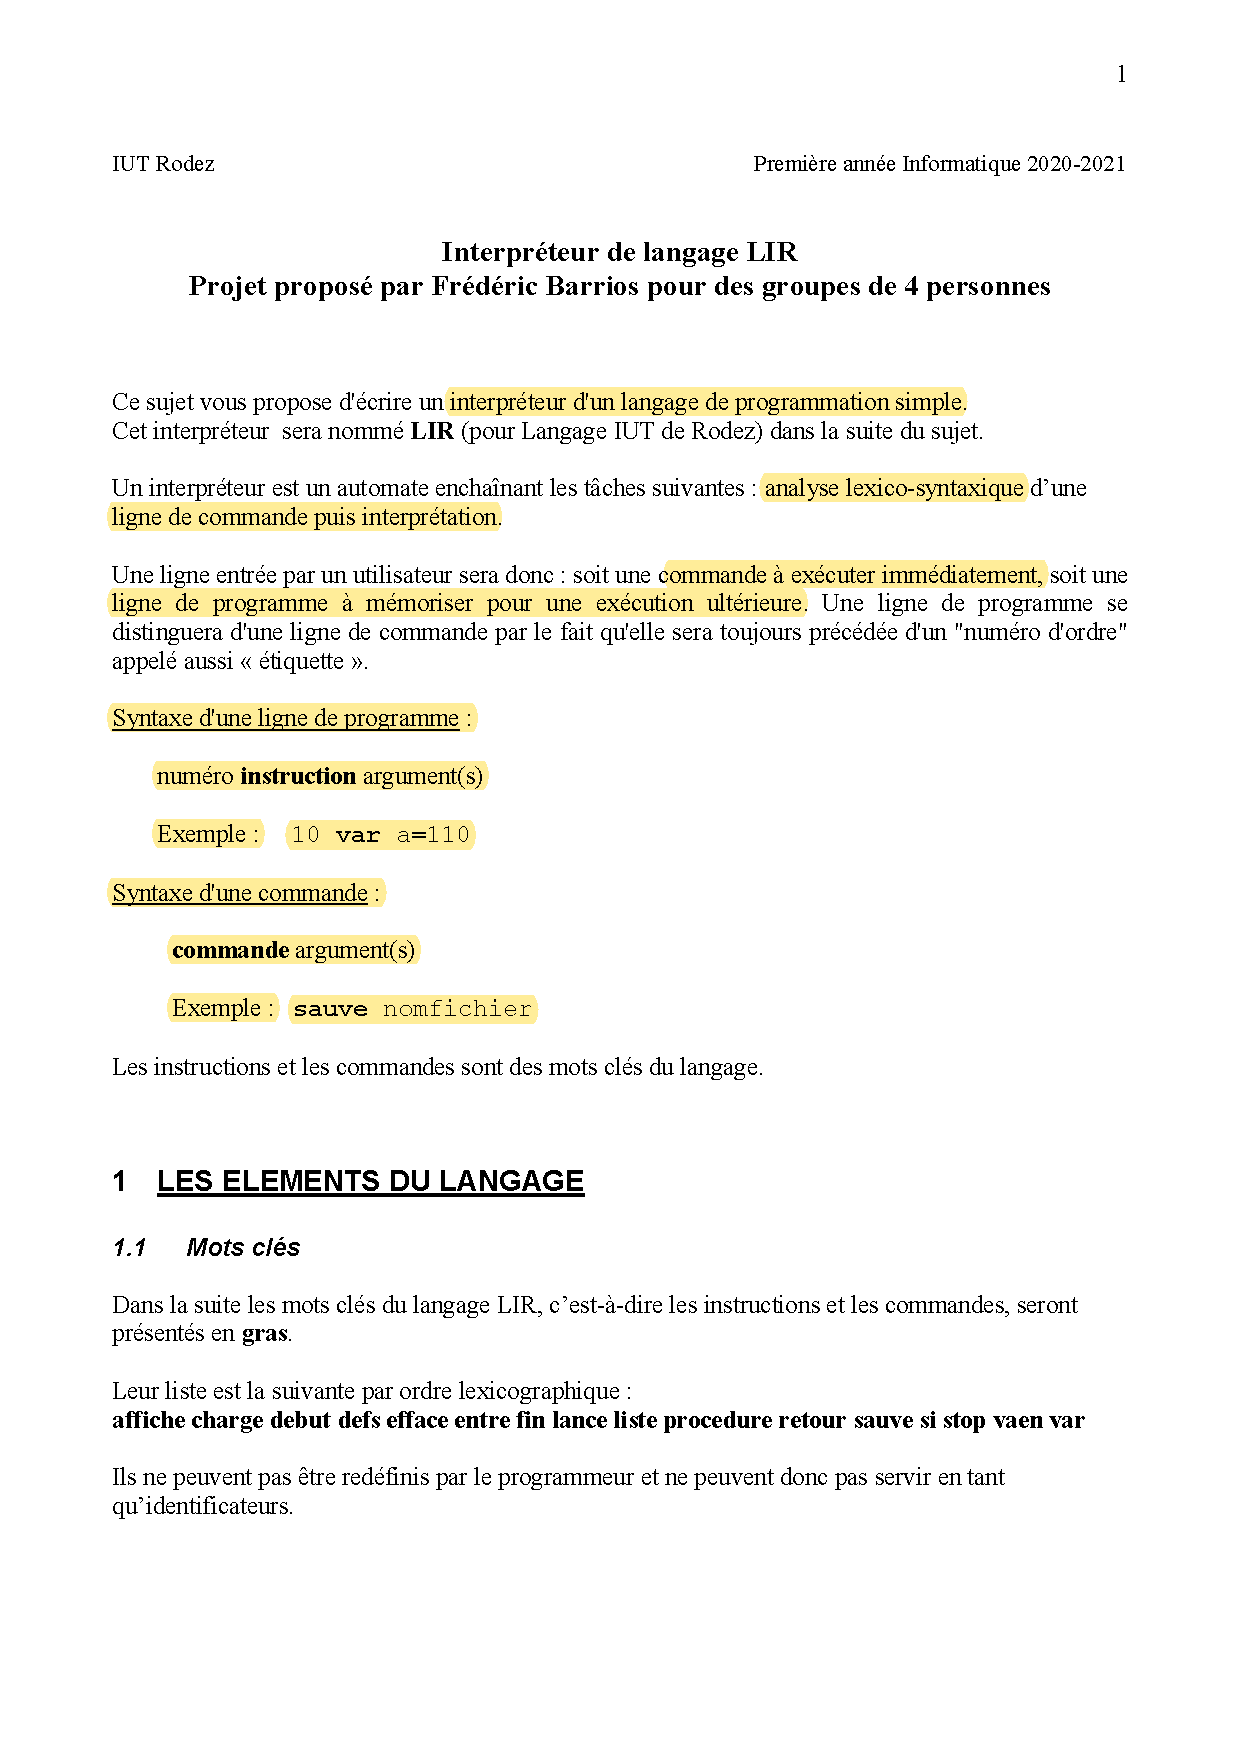
\includepdf[pages=-]{fichiers/BarriosInterpreteurLIR2021}
    \chapter{Sujet Interpréteur LIR}

    \documentclass[11pt,a4paper,titlepage,openright]{report}
\usepackage[utf8]{inputenc}
\usepackage[T1]{fontenc}
\usepackage[french]{babel}
\usepackage[top=1.5cm, bottom=5cm]{geometry}
\usepackage{fancyhdr, graphicx, array, hyperref}
\usepackage{glossaries}

\pagestyle{fancy}

\title{\textsc{\textbf{Gestion de la configuration\\Interpréteur du langage LIR}}}
\date{}
\author{Nicolas \textsc{Caminade} \and Sylvan \textsc{Courtiol} \and Pierre \textsc{Debas} \and Heïa \textsc{Dexter} \and Lucàs \textsc{Vabre} }
\begin{document}
    \lhead{Gestion de la configuration}
    \rhead{
        
\includegraphics[width=2cm]{img/logoiut}
    }

    \cfoot{\thepage}
    \headheight = 2cm
    \headsep = 1.5cm


    \begin{titlepage}
        \fontfamily{pag}\selectfont

        \begin{center}\normalsize
            \MakeUppercase{IUT de Rodez \hfill Département informatique \hfill INFO1 2020-2021}
        \end{center}
        \vspace*{0.1cm}
        \hrule
        \vspace*{0.2cm}
        \begin{flushright}
            
\includegraphics[width=4cm]{img/logoiut}
        \end{flushright}
        \vspace*{2cm}
        \begin{flushright}\Huge
            \textsc{\textbf{Gestion de la configuration\\Interpréteur du langage LIR}}
        \end{flushright}
        \hrule
        \begin{flushleft}
            \MakeUppercase{Projet proposé par Frédérique Barrios}
        \end{flushleft}
        \vspace*{1cm}
        \begin{center}\normalsize
        	\textbf{version : \today}
        \end{center}
        \vspace*{1cm}
        \begin{center}\Large
            Nicolas \textsc{Caminade}, Sylvan \textsc{Courtiol},\\
            Pierre \textsc{Debas}, Heïa \textsc{Dexter}, \\
            Lucàs \textsc{Vabre}
        \end{center}
        \vfill
        \begin{center}\normalsize
            \MakeUppercase{Projet tuteuré --- Semestre 2}
        \end{center}
    \end{titlepage}


    % Sommaire
    \renewcommand{\contentsname}{Sommaire}
    \tableofcontents
    
    \newpage

    % numérotation des sections et sous-section indiféremment des chapitres
    \setcounter{section}{0}
    \renewcommand{\thesection}{\arabic{section}} 
    \renewcommand{\thesubsection}{\arabic{section}.\arabic{subsection}}
    
    
    \section*{Introduction}
    \Large
    Ce document a pour but de confirmer par écrit la configuration logicielle choisie pour le
    projet.
    \par Le contenu de ce document n’est pas fixé et des changements peuvent être apportés. Cependant ce document doit être connu et suivi par les membres du groupe. En cas de modifications, une annonce sur discord sera faite.
    \par Pour toute question ou suggestion se référer au gestionnaire de configuration (présentement
    Sylvan COURTIOL).


    \normalsize
    \section{Logiciels de développement}
        \subsection{Environnement de Développement Intégré}
        Eclipse JEE (version 2020-12)
        \par JDK 15
        
        \subsection{Contrôle des versions du code}
        Git (notamment intégré à Eclipse) avec dépôt sur GitHub. (Un apprentissage est nécessaire
        donc pour commencer certaines libertés sont possibles).
        
        \subsection{Organisation}
        Via le site Trello (non utilisé pour le moment).
        
    \section{Logiciels généraux}
        \subsection{Communication}
        \par Les communications formelles sont effectuées via les mails de l’IUT (généralement par le chef
        de projet) avec les autres membres du projet en CC.

        \par Serveur discord spécifique au projet pour la communication écrite ou vocale de la MOE.
        \par Google Meet pour les réunions avec les personnes autres que MOE. Adaptable à ce qui
        convient le mieux à cette personne.
        
        \subsection{Éditeur de texte}
        Le traitement de texte sera fait sous LaTex notamment avec la distribution MiKTex et l'IDE TexStudio. Les documents texte sont partagés en PDF ou version papier à la MOA/MOE  et en format modifiable .tex seulement à la MOE via la solution de partage distant des fichiers (voir sous-section suivante).
        
        \subsection{Partage distant des fichiers}
        Les partages de tous les fichiers généraux et codes sources se feront sur GitHub via le site, le logiciel GitHub desktop ou git. Il y aura également une intégration Discord informant des commits.
        
    \section{Sécurité}
    \par Si possible tous les membres du groupe auront les mêmes droits sur les fichiers communs.
    En conséquence aucun membre du groupe ne doit donner des droits sur ces fichiers à une
    personne extérieure au projet (autre que MOA).
    \par Les sauvegardes du dépôt GitHub (contenant toutes les données du projets) seront effectuées
    régulièrement (tous les 1 ou 2 jours) par le gestionnaire de configuration. Toutes données qui ne
    sont pas dans le dépôt sont à la responsabilité de chacun.
    Les sauvegardes sont enregistrée en local par le gestionnaire de configuration ainsi que sur le Google drive partagé du projet.



    \appendix
    %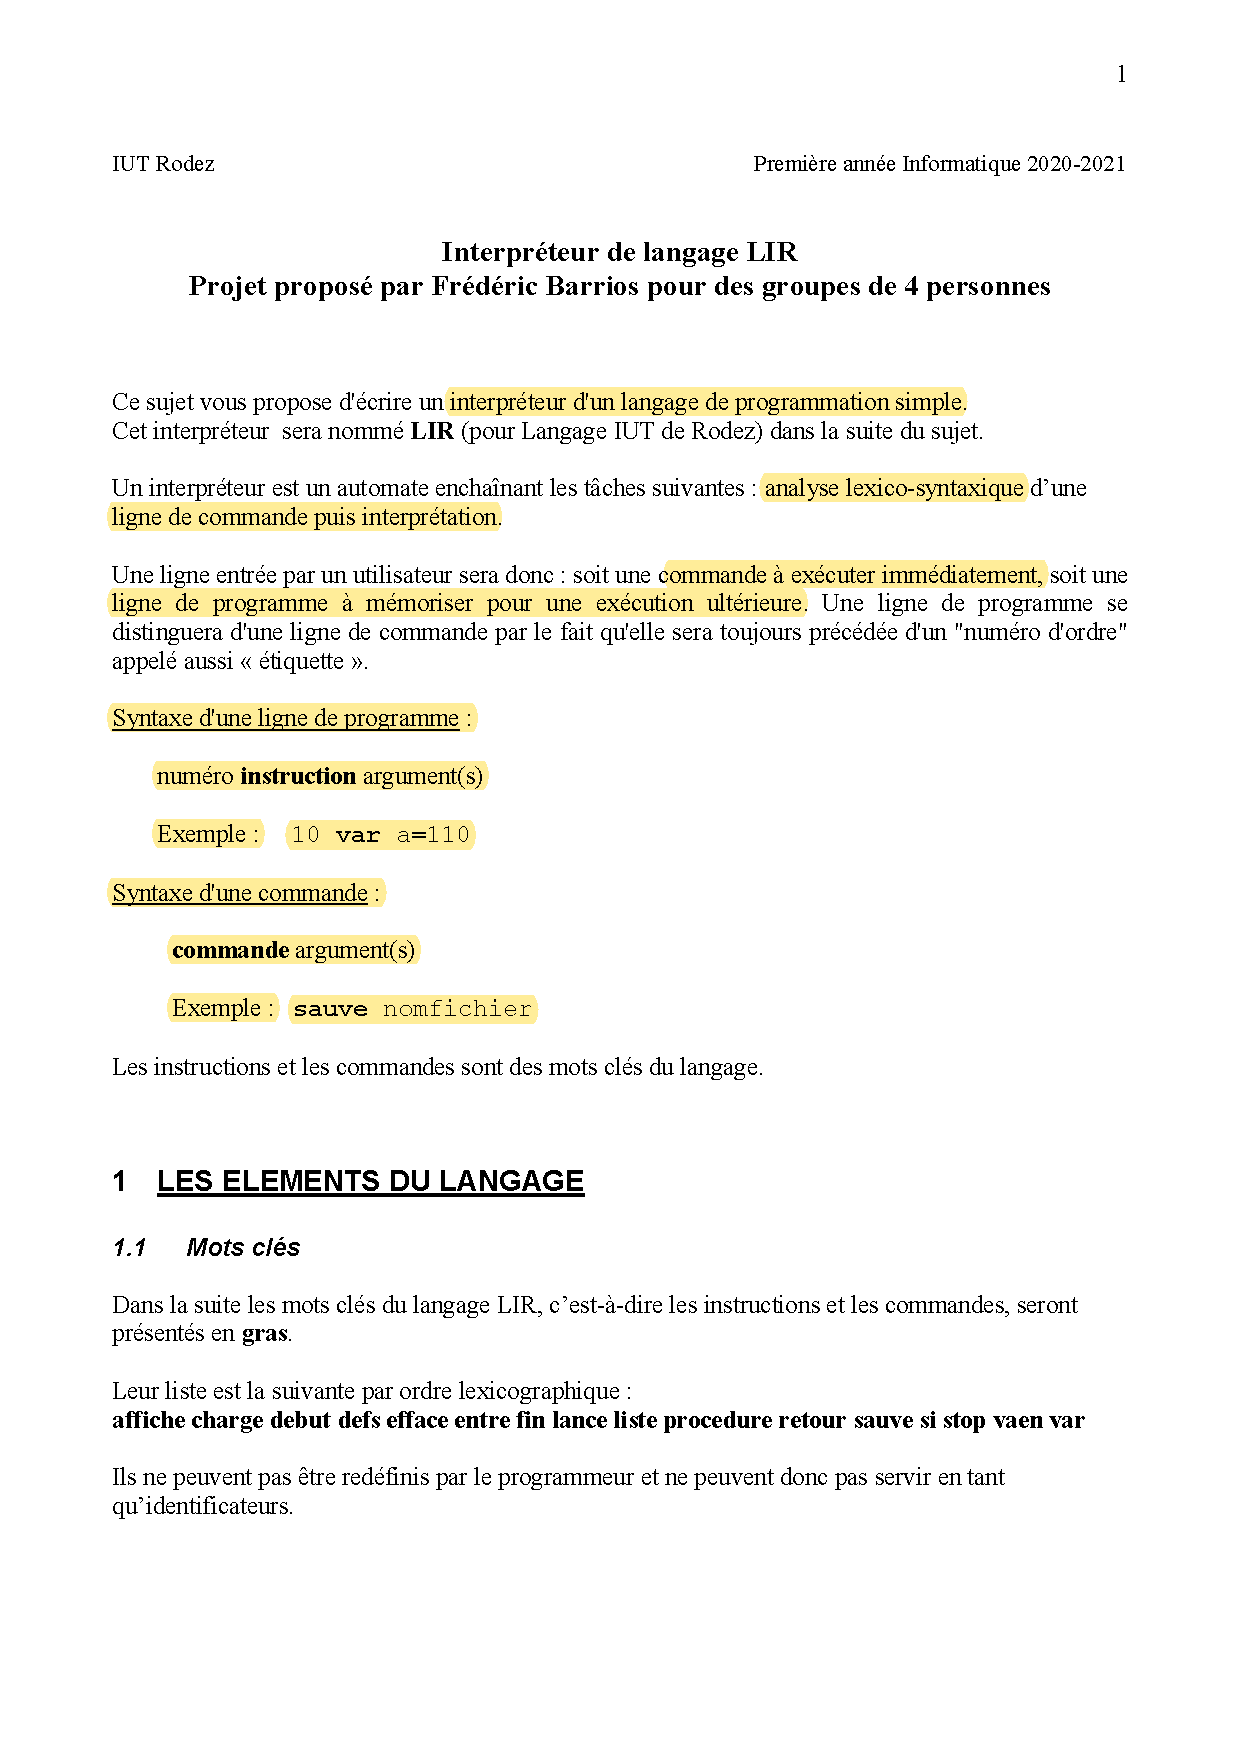
\includepdf[pages=-]{fichiers/BarriosInterpreteurLIR2021}

\end{document}

\end{document}